\begin{figure*}[t]
    \centering
    
\includegraphics[width=0.8\linewidth]{figures/abc_nn1}
    
\includegraphics[width=0.8\linewidth]{figures/abc_nn3}
    
\includegraphics[width=0.8\linewidth]{figures/abc_nn4}
    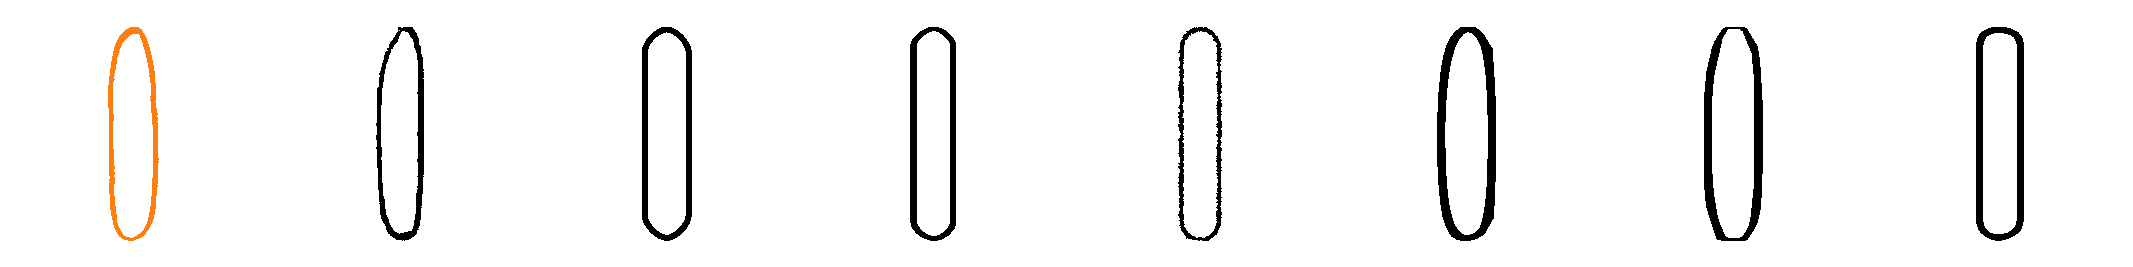
\includegraphics[width=0.8\linewidth]{figures/abc_nn6}
    \caption{Glyph nearest neighbors in curve space.}
    \label{fig:sup-nn}
\end{figure*}


\begin{figure*}[t]
    \centering
    
\includegraphics[width=0.8\linewidth]{figures/abc_interpolation1}
    
\includegraphics[width=0.8\linewidth]{figures/abc_interpolation2}
    
\includegraphics[width=0.8\linewidth]{figures/abc_interpolation5}
    
\includegraphics[width=0.8\linewidth]{figures/abc_interpolation6}
    \caption{Interpolations between fonts in curve space.}
    \label{fig:sup-interpolation} 
\end{figure*}

\begin{figure*}[t]
    \centering
    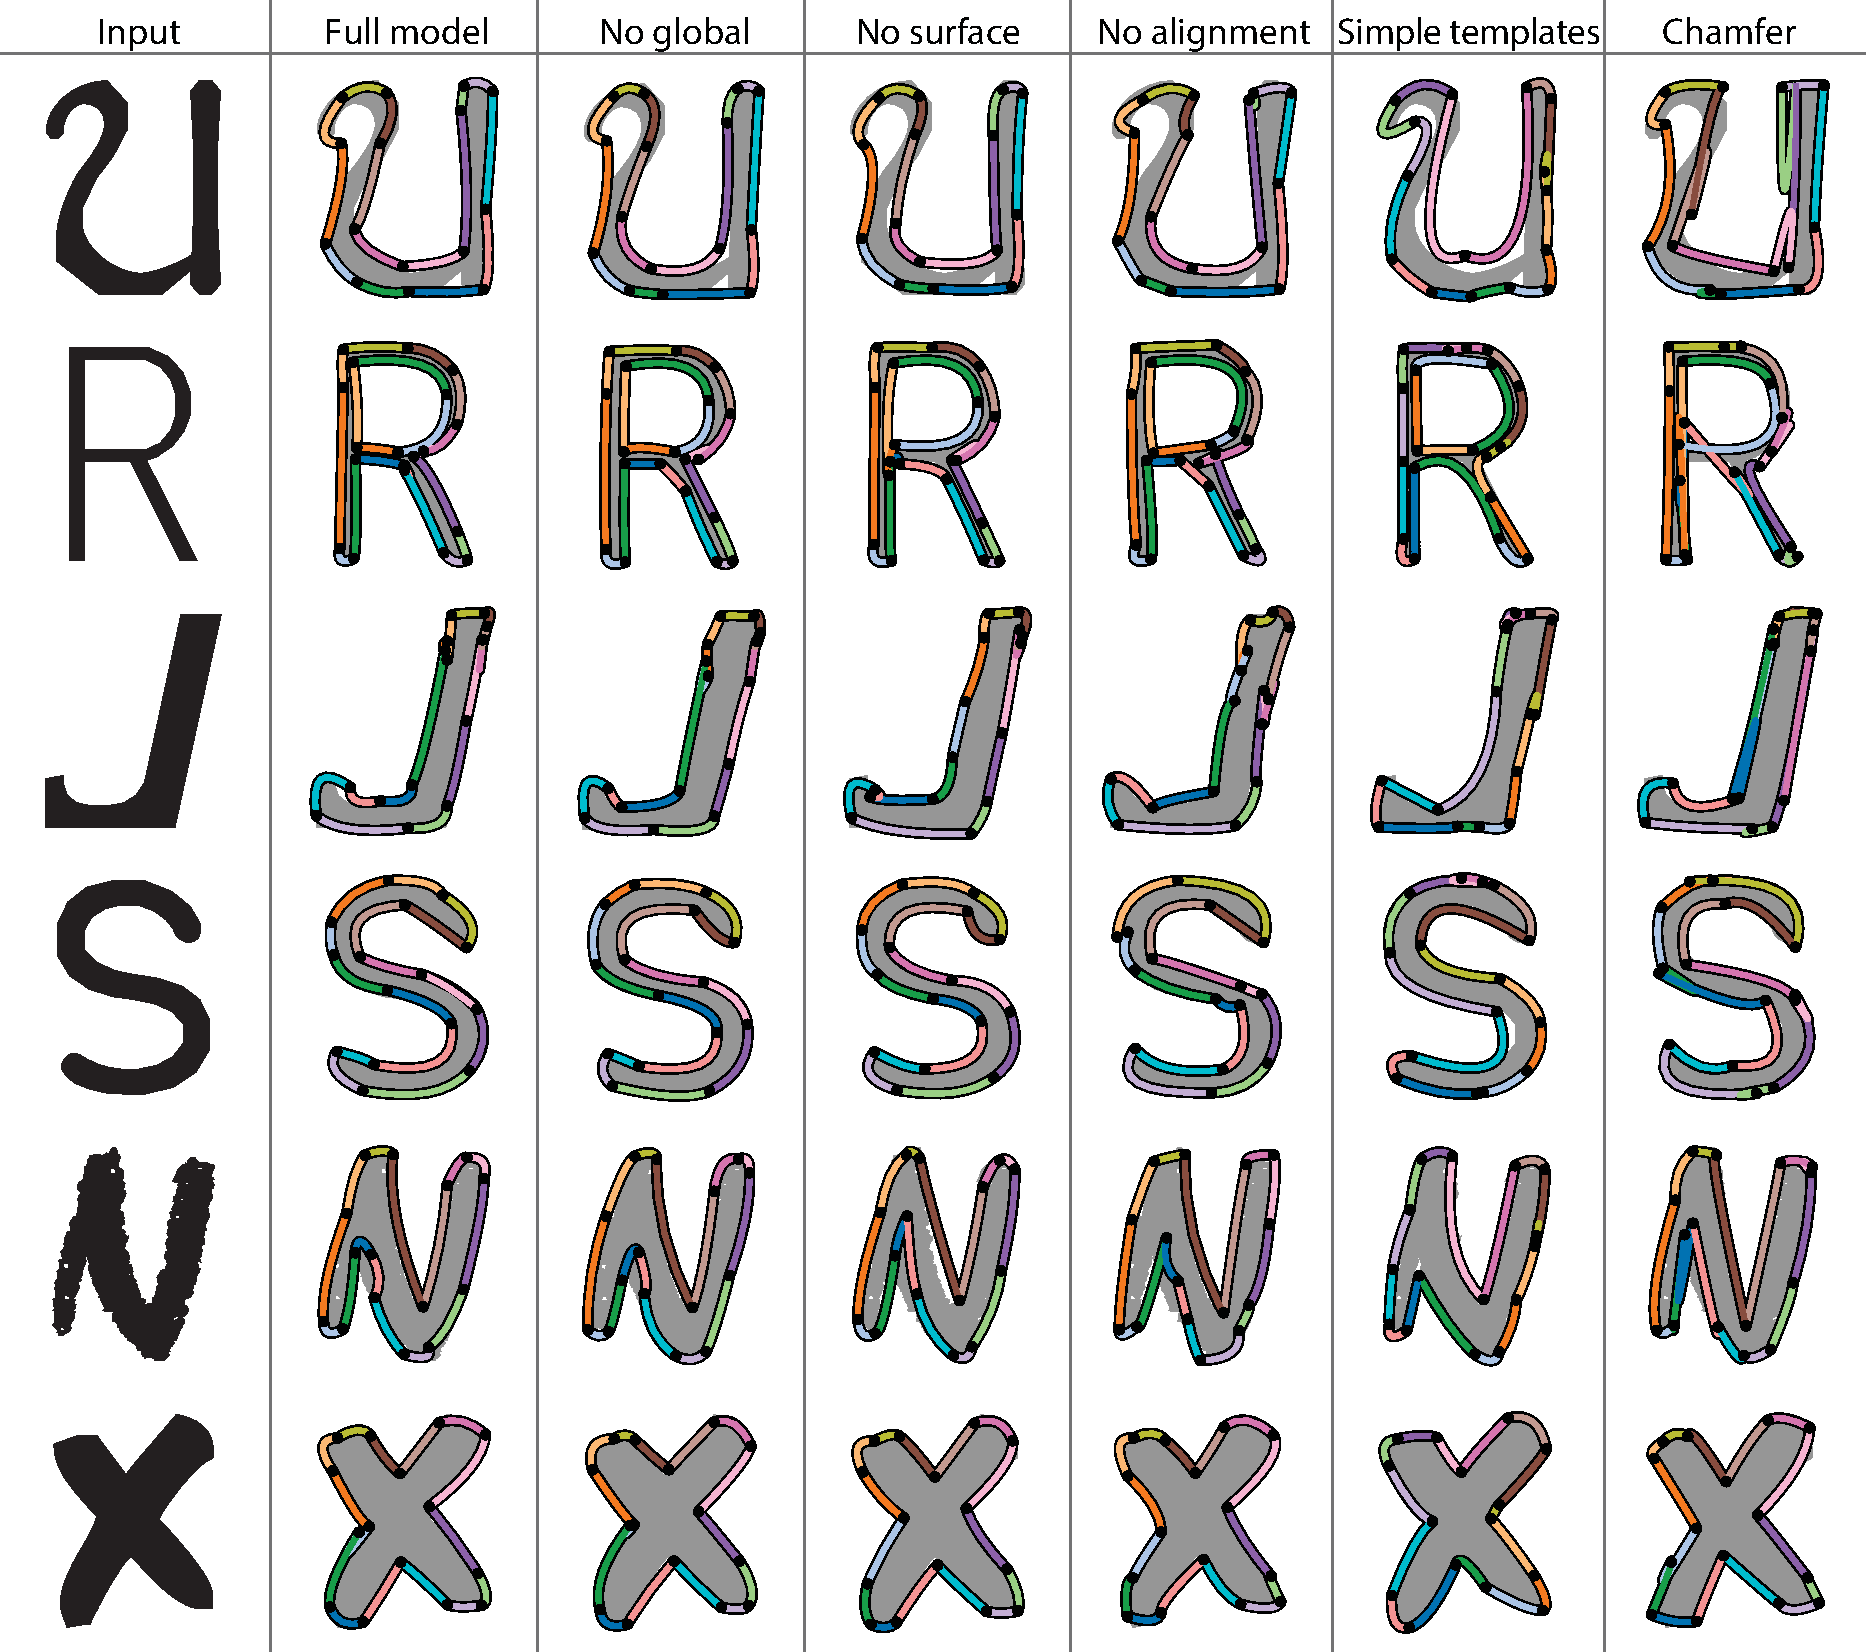
\includegraphics[width=\linewidth]{figures/sup_ablation}
    \caption{Distance field loss comparisons.}
    \label{fig:sup-ablation}
\end{figure*}

\begin{figure*}[t]
    \centering
    \includegraphics[width=.4\linewidth]{figures/loss_convergence}\vspace{-.1in}
    \caption{Local loss (smoothed) over the first 4,000 iterations of training with and without global loss in the objective function. The global loss term results in faster convergence.\vspace{-0.1in}}
    \label{fig:loss_convergence}
\end{figure*}


\begin{figure*}[t!]
    \centering
    \includegraphics[width=\linewidth]{figures/sup_chairs}
    \label{fig:sup-chairs}
    \caption{Cuboid reconstructions of ShapeNet chairs.}
\end{figure*}

\begin{figure*}[t!]
    \centering
    \includegraphics[width=\linewidth]{figures/sup_airplanes}
    \label{fig:sup-airplanes}
    \caption{Cuboid reconstructions of ShapeNet airplanes.}
\end{figure*}

\begin{figure*}[t!]
    \centering
    \includegraphics[width=0.8\linewidth]{figures/sup_seg}
    \label{fig:sup-seg}
    \caption{Cuboid segmentation of Shape COSEG chairs.}
\end{figure*}